\chapter{Project Assumptions}
\section{Overall Description}

The main goal of the project is to create a mobile application that can be connected to an API of any university. It will be done using the Flutter framework and the Dart language. The app will be ready to run on both iOS and Android devices. Every student is required to have an existing account in their university system and log in to the mobile app to access all of the functionalities. None of them can be used as an unauthenticated user. After they log in, students will gain access to these pages:

\begin{multicols}{2}
\begin{itemize}
    \item home (user details and news);
    \item calendar with a schedule;
    \item grades;
    \item messages;
    \item message details;
    \item payments.
\end{itemize}
\end{multicols}

Users cannot make changes to any data shown on the listed pages. It is obtained from their university services system and stored on their local devices as read-only information.

When a student logs in, a token received from the student service system will be saved to secure storage on the mobile device. It will be removed if the user explicitly logs out of the application. The token will be used to obtain data from the university system. It will also allow the system to store information about users and will not require them to log in each time they open the application. To log in, users will have to complete a form, where they will have to select their university from the drop-down list and provide login and password to the account in their university system.

The homepage will show user details and news from the users' faculty and university. The next page will display a calendar that users can click on to select a date. After picking the day, students will receive a list of planned lectures with specifics like start and end time, lecturer, classroom, etc. The grades and payments pages will provide a list of items with some type-specific details. The former will also allow students to calculate the overall average grade of all grades relative to the ECTS weighting of the courses they have completed. The last one is the messages page. It will present all messages received by users in their university system. After they select one of the e-mails, they will be redirected to a more detailed view.

\section{Functional Requirements}
% TO DO: proszę dodać jakieś wprowadzenie (np. Poniżej zebrano wymagania funkcjonalne, które .... Funkcje dostępne dla użytkownika zebrano na przedstawionym dalej diagramie przypadków użycia)
\begin{itemize}
    \item The software system should be integrated with university APIs.
    \item The system will translate JSON from the mobile application request into JSON compatible with the university API.
    \item The software automatically validates customers against the university API.
    \item The system will limit access to authorized users.
    \item Users should be able to browse calendars and calendar events.
    \item Users should be able to view the grades list.
    \item The system should allow users to calculate their average grade.
    \item Users should be able to browse messages.
    \item Users should be able to see message details.
    \item Users should be able to browse the payments list.
    \item Users should be able to see the news feed.
    \item Users should be able to view user details.
    \item Every user has to have an account in one of the available university systems.
\end{itemize}

\section{Non-functional Requirements}
% TO DO: proszę dodać jakieś wprowadzenie (np. Poniżej zebrano wymagania niefunkcjonalne, które .....)
\begin{itemize}
    \item The system will be composed of 3 layers: mobile database, mobile application, and transformation server.
    \item The mobile SQLite database will store user data, grades, calendar events, payments, and messages.
    \item The mobile application will support Polish and English.
    \item The transformation server will be created using the Java language and Spring Framework.
    \item The server will use Spring Boot to accelerate the preparation and configuration.
    \item The transformer will utilize Spring Could Config to provide a dynamic and simple way to update the university API configurations. The server will not have to be restarted to apply new settings because they will refresh automatically.
    \item The configuration will be served as YAML files.
    \item All requests will utilize the JSON format.
    \item The transformation specification will use JSON format and will be handled by the Jolt library.
    \item The authentication will be managed by the server and the university's external API.
    \item The mobile application will be made using the Dart language and Flutter framework. It will allow generating two applications for both iOS and Android, using one codebase.
    \item MockServer will be used to mock the external API to which the transformation server will send requests. It will ease the development and speed up testing.
    \item Docker Compose will be used to define and run multi-container Docker applications, in this case, the transformation server and its configuration.
    \item Version control will be supported by Git and GitHub platforms.
    \item All tasks and issues will be managed with GitKraken Glo Board.
    \item All development will be done using Android Studio IDE.
\end{itemize}

\section{Use Cases}
A use case diagram (Fig.~\ref{fig:use-case-diagram}) represents the main functionalities available to users. All of them require users to be authenticated. The diagram is simplified and does not contain connections between the "Authenticate/Authorize" use case and all the others.

% TO DO: diagram jest "za rzadki" (ma za dużo białej przestrzeni, owale są za duże względem tekstu)
\begin{figure}[htb]
    \centering
    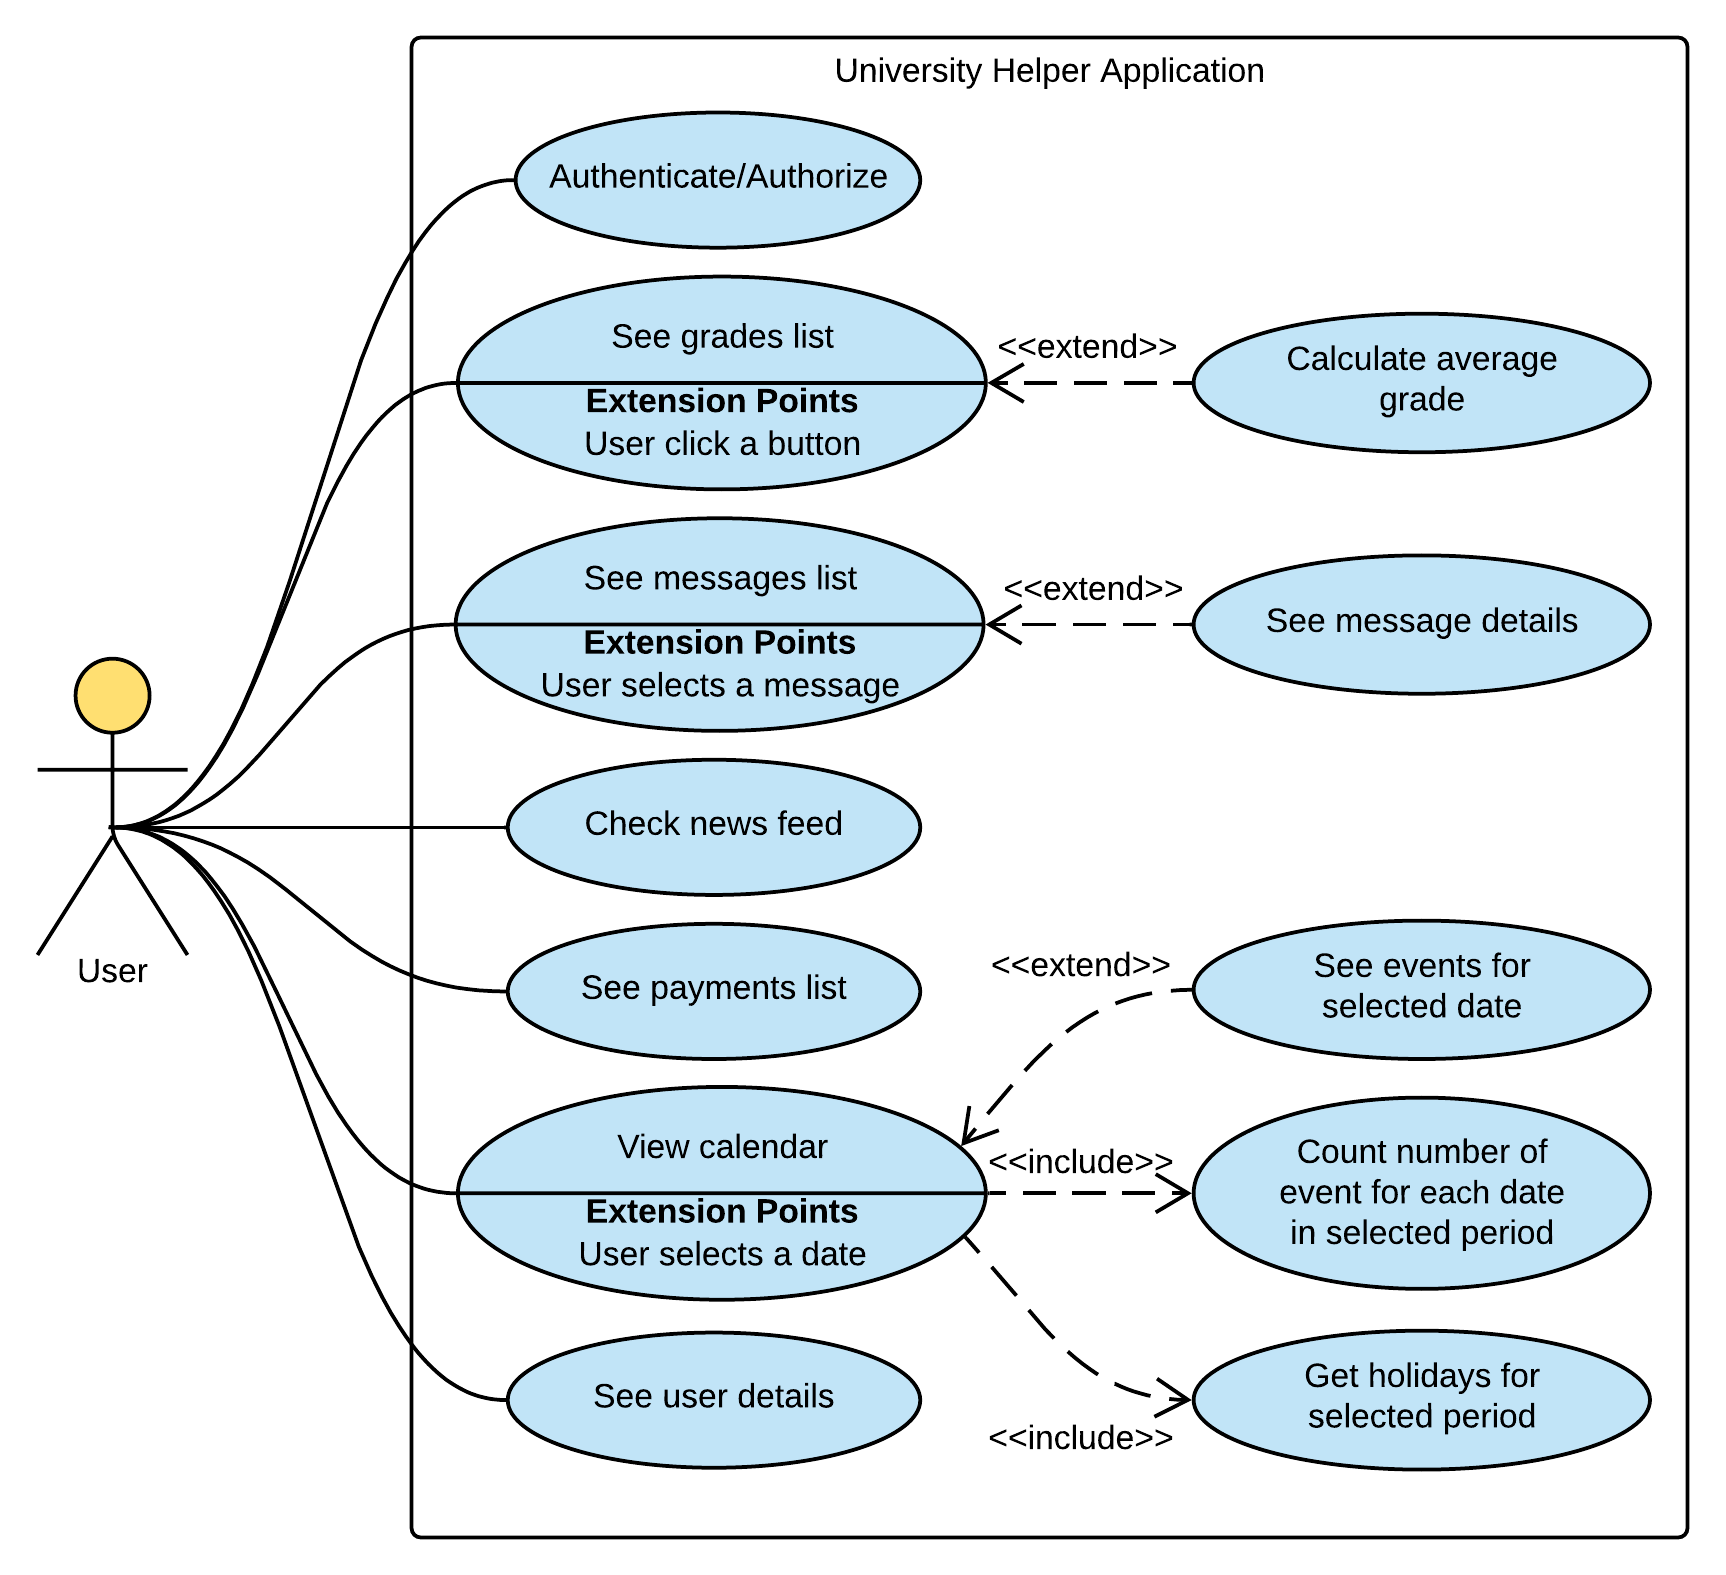
\includegraphics[width=\textwidth]{fig02/use_case_diagram.png}
    \caption{Use case diagram} \label{fig:use-case-diagram}
\end{figure}

% ---------------------------------------------

\paragraph{\large{Authenticate/Authorize}}\mbox{}\\[2pt]
\textbf{Primary Actor:} User\\
\textbf{Scope:} Mobile application\\
\textbf{Level:} Fish level\\
\textbf{Brief:} The user logs in to the mobile application.\\
\textbf{Trigger:} The user open the mobile application.\\
\textbf{Preconditions:}
The user has an account in one of the available university systems.\\
\textbf{Basic flow:}
\begin{enumerate}
    \item The system's login screen has a drop-down with available universities.
    \item The user chooses her/his university and enter credentials.
    \item The user submits the form.
    \item The mobile application sends the credentials to the server.
    \item The server validates the credentials and sends a response back to the mobile application.
    \item The system redirects the user to the homepage.
\end{enumerate}
\textbf{Postconditions:}
The user is authenticated and can access all screens of the mobile application.

% ---------------------------------------------

\paragraph{\large{See grades list}}\mbox{}\\[2pt]
\textbf{Primary Actor:} User\\
\textbf{Scope:} Mobile application\\
\textbf{Level:} Sea level\\
\textbf{Brief:} The user wants to see her/his grades.\\
\textbf{Trigger:} The user selects "Grades" screen from the mobile application.\\
\textbf{Preconditions:}
\begin{itemize}
    \item The user has an account in one of the available university systems.
    \item The user is authenticated.
\end{itemize}
\textbf{Basic flow:}
\begin{enumerate}
    \item The system redirects the user to the "Grades" page.
    \item The mobile application sends a request to the server.
    \item The server fetches data from the university system and sends a response back to the mobile application.
    \item The mobile application loads the data and refreshes the view with the list of grades.
\end{enumerate}
\textbf{Postconditions:}
The user can see the list of her/his grades.\\
\textbf{Extensions:}
\begin{enumerate}[label=\alph*.]
    \item Calculate average grade:
    \begin{enumerate}
        \item The user clicks on the "Calculate average" button.
        \item The system calculates an average grade for all semesters and displays it to the user.
    \end{enumerate}
\end{enumerate}

% ---------------------------------------------

\paragraph{\large{See messages list}}\mbox{}\\[2pt]
\textbf{Primary Actor:} User\\
\textbf{Scope:} Mobile application\\
\textbf{Level:} Sea level\\
\textbf{Brief:} The user wants to see her/his messages.\\
\textbf{Trigger:} The user selects "Messages" screen from the mobile application.\\
\textbf{Preconditions:}
\begin{itemize}
    \item The user has an account in one of the available university systems.
    \item The user is authenticated.
\end{itemize}
\textbf{Basic flow:}
\begin{enumerate}
    \item The system redirects the user to the "Messages" page.
    \item The mobile application sends a request to the server.
    \item The server fetches data from the university system and sends a response back to the mobile application.
    \item The mobile application loads the data and refreshes the view with the list of messages.
\end{enumerate}
\textbf{Postconditions:}
The user can see the list of her/his messages.\\
\textbf{Extensions:}
\begin{enumerate}[label=\alph*.]
    \item See message details:
    \begin{enumerate}
        \item The user selects a message from the list.
        \item The system redirects the user to a page showing message details.
    \end{enumerate}
\end{enumerate}

% ---------------------------------------------

\paragraph{\large{See payments list}}\mbox{}\\[2pt]
\textbf{Primary Actor:} User\\
\textbf{Scope:} Mobile application\\
\textbf{Level:} Sea level\\
\textbf{Brief:} The user wants to see her/his payments.\\
\textbf{Trigger:} The user selects "Payments" screen from the mobile application.\\
\textbf{Preconditions:}
\begin{itemize}
    \item The user has an account in one of the available university systems.
    \item The user is authenticated.
\end{itemize}
\textbf{Basic flow:}
\begin{enumerate}
    \item The system redirects the user to the "Payments" page.
    \item The mobile application sends a request to the server.
    \item The server fetches data from the university system and sends a response back to the mobile application.
    \item The mobile application loads the data and refreshes the view with the list of payments.
\end{enumerate}
\textbf{Postconditions:}
The user can see the list of her/his payments.

% ---------------------------------------------

\paragraph{\large{Check news feed}}\mbox{}\\[2pt]
\textbf{Primary Actor:} User\\
\textbf{Scope:} Mobile application\\
\textbf{Level:} Sea level\\
\textbf{Brief:} The user wants to see news from her/his faculty and university.\\
\textbf{Trigger:} The user goes to the homepage of the mobile application.\\
\textbf{Preconditions:}
\begin{itemize}
    \item The user has an account in one of the available university systems.
    \item The user is authenticated.
\end{itemize}
\textbf{Basic flow:}
\begin{enumerate}
    \item The system redirects the user to the homepage.
    \item The mobile application sends a request to the server.
    \item The server fetches news from the university system and sends a response back to the mobile application.
    \item The mobile application loads the data and refreshes the news feed section.
\end{enumerate}
\textbf{Postconditions:}
The user can see the list of news in the news feed section of the homepage.

% ---------------------------------------------

\paragraph{\large{View calendar}}\mbox{}\\[2pt]
\textbf{Primary Actor:} User\\
\textbf{Scope:} Mobile application\\
\textbf{Level:} Sea level\\
\textbf{Brief:} The user wants to see her/his calendar.\\
\textbf{Trigger:} The user selects "Calendar" screen from the mobile application.\\
\textbf{Preconditions:}
\begin{itemize}
    \item The user has an account in one of the available university systems.
    \item The user is authenticated.
\end{itemize}
\textbf{Basic flow:}
\begin{enumerate}
    \item The system redirects the user to the "Calendar" page.
    \item The mobile application sends a request to the server.
    \item The server fetches data from the university system and sends a response back to the mobile application.
    \item The mobile application loads the data and refreshes the calendar with the list of events.
\end{enumerate}
\textbf{Postconditions:}
The user can see her/his calendar.
\textbf{Extensions:}
\begin{enumerate}[label=\alph*.]
    \item See events for selected date:
    \begin{enumerate}
        \item The user selects a date from the calendar.
        \item The system shows a list of events for the selected date.
    \end{enumerate}
\end{enumerate}

% ---------------------------------------------

\paragraph{\large{Get holidays for selected period}}\mbox{}\\[2pt]
\textbf{Primary Actor:} User\\
\textbf{Scope:} Mobile application\\
\textbf{Level:} Fish level\\
\textbf{Brief:} Get holidays from an external API for a selected period.\\
\textbf{Trigger:} The user selects "Calendar" screen from the mobile application or chooses another period.\\
\textbf{Preconditions:}
\begin{itemize}
    \item The user has an account in one of the available university systems.
    \item The user is authenticated.
\end{itemize}
\textbf{Basic flow:}
\begin{enumerate}
    \item The mobile application sends a request to the external API.
    \item The external API sends a response with a list of holidays for the selected period.
    \item The mobile application loads the data and refreshes the calendar with the list of holidays.
\end{enumerate}
\textbf{Postconditions:}
Holidays for the selected period are loaded into the system and shown on the calendar page.

% ---------------------------------------------

\paragraph{\large{Count number of event for each date in selected period}}\mbox{}\\[2pt]
\textbf{Primary Actor:} User\\
\textbf{Scope:} Mobile application\\
\textbf{Level:} Fish level\\
\textbf{Brief:} Count events for every date in the selected period.\\
\textbf{Trigger:} The user selects "Calendar" screen from the mobile application or chooses another period.\\
\textbf{Preconditions:}
\begin{itemize}
    \item The user has an account in one of the available university systems.
    \item The user is authenticated.
    \item The calendar events are stored in the system.
\end{itemize}
\textbf{Basic flow:}
\begin{enumerate}
    \item The mobile application loads events for each date in the selected period.
    \item The mobile application counts all events and refreshes the calendar with the number of events per day.
\end{enumerate}
\textbf{Postconditions:}
The number of events for each day in the selected period is shown on the calendar page.

% ---------------------------------------------

\paragraph{\large{See user details}}\mbox{}\\[2pt]
\textbf{Primary Actor:} User\\
\textbf{Scope:} Mobile application\\
\textbf{Level:} Sea level\\
\textbf{Brief:} The user wants to see profile details.\\
\textbf{Trigger:} The user goes to the homepage of the mobile application.\\
\textbf{Preconditions:}
\begin{itemize}
    \item The user has an account in one of the available university systems.
    \item The user is authenticated.
\end{itemize}
\textbf{Basic flow:}
\begin{enumerate}
    \item The system redirects the user to the homepage.
    \item The mobile application sends a request to the server.
    \item The server fetches user data from the university system and sends a response back to the mobile application.
    \item The mobile application loads the data and refreshes the profile info section.
\end{enumerate}
\textbf{Postconditions:}
The user can see the profile details section on the homepage.
